\section{Theoretical Background}
Fabrication techniques such as electron beam lithography (EBL) are used to produce the GaAs/AlGaAs heterostructure. The heterostructure enables a small number of free electrons, with the DeBroglie wavelengths similar to the QD size, to be confined in a quantum well \citen{BoscoQuantumEffect}. The electrons between the GaAs and AlGaAs semi-conducting surfaces act as a 2-dimensional electron gas (2DEG) [\citen{Ihn2009SemiconductorNanostructures,Kouwenhoven1997IntroductionTransport}]. Etching gate electrodes on the surface of the GaAs layer enables controlled confinement of the electrons to 3-dimensions. Therefore these artificial atoms result in electrons occupying discrete energy levels, observed at low temperatures, which follow atomic physics rules. Therefore, quantum dot devices are contained within a dilution refrigerator where the electrons are kept at $\approx100$ mK temperatures during experiments [\citen{Petta2004ManipulationDot}]. 

The Coulomb repulsion between electrons must be overcome to add an additional electron to the dot. The electro-chemical potential is the energy difference between the single dot ground state containing $N$ and $N+1$ electrons: 

\begin{equation}
\label{eq:interactionham0}
\mu (N) = -\frac{E_{C}}{\left | e \right |}(C_{S}V_{S}+C_{D}V_{D}+C_{G}V_{G})+E_{N}, 
\end{equation}

where charging energy to cross the junction into the dot is $E_{C}=\frac{e^{2}}{C}$. The total capacitance $C$ is the sum of the capacitance of the source, drain and gate electrodes which are $C_{S}, C_{D}$, and $C_{G}$, respectively. Similarly for the applied electron voltages, $V_{S}, V_{D}$ and $V_{G}$ as shown in Fig. (\ref{fig:QDaa}). The chemical potential energy of Nth additional electron is $E_{N}$. The additional energy is thus given as: 

\begin{equation}
\label{eq:interactionham0}
E_{add}(N)=\mu(N+1)-\mu(N)=E_{C}+E_{N+1}-E_{N},
\end{equation}

where spin filling resulting from the Pauli exclusion principle dictates the value of $E_{N+1}-E_{N}$ being zero or nonzero [\citen{Hanson2007SpinsDots}]. 
 
\begin{figure}[t]
\centering
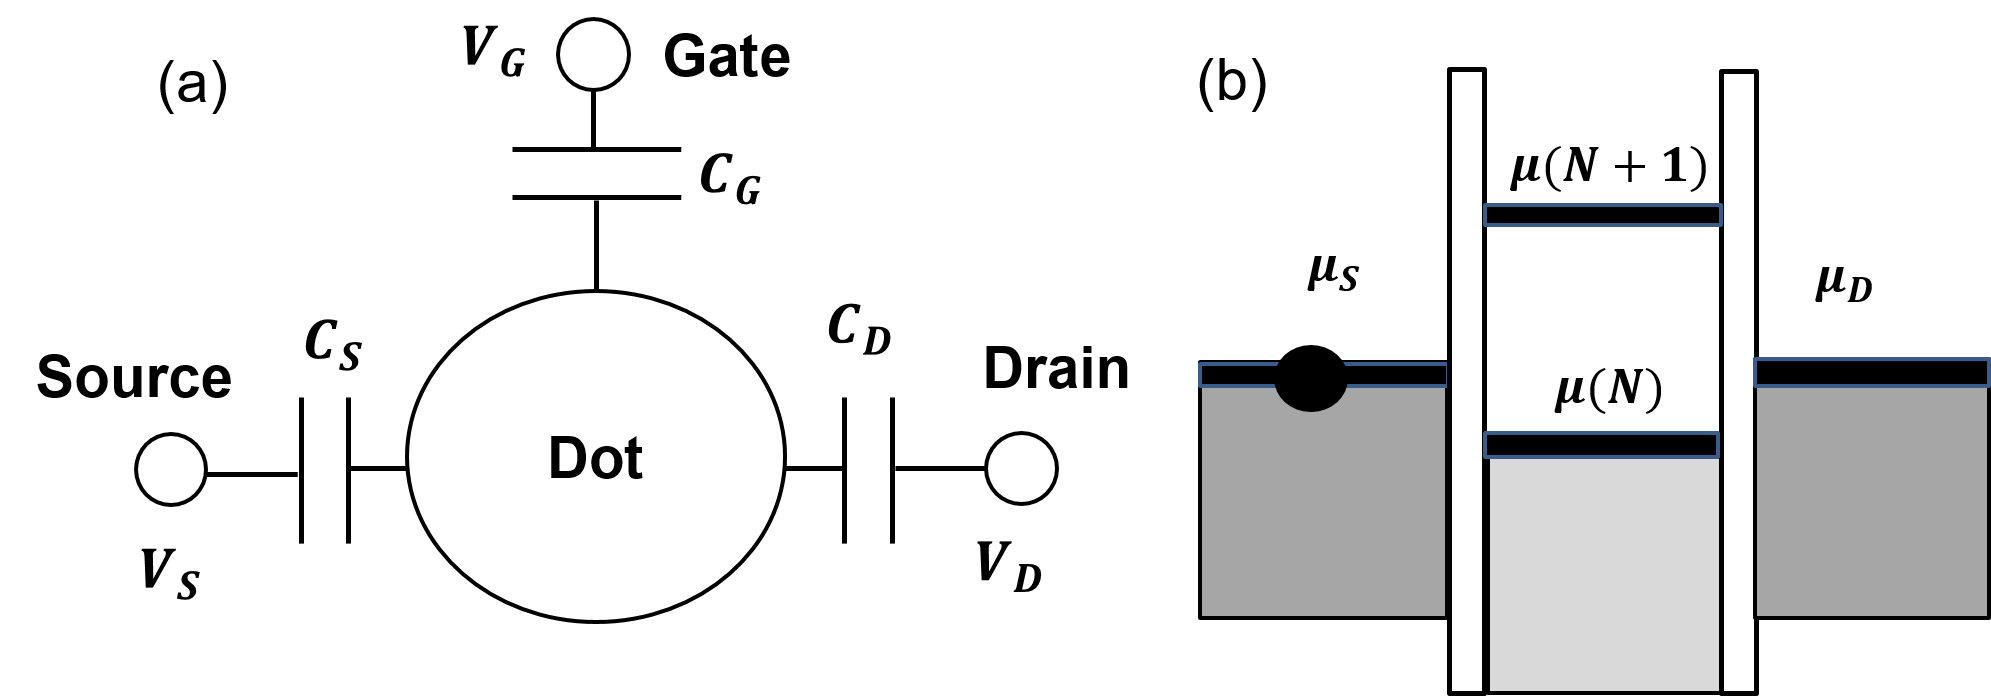
\includegraphics[height=0.18\textwidth,keepaspectratio]{QDaa}
\caption{\label{fig:QDaa}(a) Single QD schematic showing electrode connections. (b) Energy level diagram with the Coulomb blockade condition satisfied.}
\end{figure} 

Controlling of voltage of the electrodes allows electrons to tunnel into the QD. The Coulomb blockade refers to the case where $\mu_{S} \geq \mu(N) \geq \mu_{D}$ and the QD electron number is constant. Extension of this derivation to include double QDs is given in Ref. [\citen{vanderWiel2002ElectronDots}] where each dot has a individual plunger gate electrode. An additional gate electrode of voltage $V_{M}$ separates the dots. Double quantum dots enable encoding of the charge or spin degree of freedom of the qubit. 
  

  


